\documentclass[11pt]{article}

\usepackage{amsmath, amssymb, amsthm, mathrsfs, euler}
\usepackage{enumerate}
\usepackage[margin = 1in]{geometry}
\usepackage{graphicx}
\usepackage{float}

\usepackage{../defs}
\usepackage{../thmdefs}

\title{Application of Convex Relaxation on Low-rank Optimization Problems}
\author{GKxx, YHZ, ZYP}
\date{\today}

\begin{document}

\maketitle

\tableofcontents

\newpage

\section{An introduction for convex relaxation}

In research, plenty of traditional methods for solving non-convex optimization problems have been found and have proved effective. Some of them are listed below.

\begin{enumerate}
    \item Block coordinate descent method\par
    In each generation selection process, only one variable is optimized and solved, while the rest variables remain unchanged and then solved alternately.
    \item Successive convex approximation method\par
    The first order Taylor expansion of the objective function was carried out at a fixed point, and then the approximate function was constructed to solve the problem instead of the original objective function.
    \item Convex relaxation method\par
    A relaxation variable or function is introduced to replace some part of the original objective function with, so that the objective function becomes convex and the problem reduces to a convex problem.
\end{enumerate}

In this project, we mainly focus on the third method. The core idea of convex relaxation is to transform an arbitrary non-convex problem into a convex one, which has more desired properties. An ideal relaxation is supposed to ensure that the optimal solution is the same as that of the original problem, while this might be difficult to achieve in practice. In the next section, we will look at a classic example in which a convex relaxation has been found and is good enough to ensure that the optimal solution remains unchanged.

\section{Low-rank Optimization}

\subsection{Introduction}

Recently, low-rank problems, such as affine constrained rank minimization problems (ARMP), have received considerable attention from the computer vision communities, among many other research communities in science and engineering. In the area of computer vision, a wide range of problems can be, and have been, represented under this low-rank or rank-minimization framework. Low-rank models have been used to interpret/approximate in high dimension and for large scale measurements. The low-rank formulation seems to be able to effectively capture the low-order structure of the underlying problems.

In general, a low-rank problem is to optimize the rank of a matrix with a series of constraints. We first show some examples of problems of this kind.

\begin{example}
    In non-rigid structure-from-motion (NRSfM), a recent work by Dai \emph{et al.} \cite{dai2014simple} showed that under rank minimization formulation to NRSfM factorization
    \[\begin{aligned}
        \minimize & \rank(S^{\sharp})\\
        \subjectto & W=RS\\
        & S^{\sharp}:=\bvec{P_X & P_Y & P_Z}\left(I_3\otimes S\right)=g(S),
    \end{aligned}\]
    there exist configurations such that multiple solutions explain the same measurements exactly.
\end{example}

\begin{example}\label{eg:latlrr}
    Latent low rank representation (LatLRR) model:
    \[\begin{aligned}
        \minimize & \rank Z+\rank L\\
        \subjectto & X=XZ+LX.
    \end{aligned}\]
    The nuclear norm minimization formulation for LatLRR is:
    \[\begin{aligned}
        \minimize & \norm Z_\ast+\norm L_\ast\\
        \subjectto & X=XZ+LX.
    \end{aligned}\]
    By analyzing the noiseless LatLRR model, Zhang \emph{et al.} \cite{zhang2013counterexample} showed that for this rank minimization problem the validity of replacing rank minimization with nuclear norm minimization may still break down. Furthermore, they proved that the solution to the nuclear norm minimization formulation of LatLRR is non-unique \cite{dai2014rank}.
\end{example}

Although in Example \ref{eg:latlrr} the nuclear norm does not provide an effective relaxation, it still works well as convex relaxation under particular conditions, which is our main topic.

\subsection{Equality Constraints}

First, we consider a standard form of low-rank problem, which has only one linear equality constraint.
\begin{definition}[Low-rank minimization]\label{def:lowrank}
    Let \(\mathcal{A}:\R^{m\by n}\to \R^p\) be a linear map and \(b\in \R^p\), the \emph{low-rank minimization} problem is of the form 
    \[\begin{aligned}
        \minimize & \rank X\\
        \subjectto & \mathcal A(X)=b.
    \end{aligned}\]
\end{definition}

Clearly, \(\rank(\cdot)\) is not a convex function, then this is not a convex optimization problem, though it always has a optimal value. However, if we attach some conditions, we can find a convex problem to relax it tightly, i.e. an optimal point of the relaxed convex problem is also an optimal point of the original problem. Now, we define some notations:

\begin{definition}[Support]
    The \emph{support} of a vector x is defined as
    \[\supp(x) = \left\{i \mid x_i \neq 0\right\}.\]
\end{definition}

\begin{definition}[Approximately sparse vectors]
    \emph{The set of approximately sparse vectors} with support \(S\) is 
    \[C(S):=\left\{\Delta \in \R^d \mid \norm{\Delta_{\bar{S}}}_1\leqslant \norm{\Delta_S}_1\right\},\]
    where \(S\) is a subset of \([d]:=\{1,2,\cdots,d\}\), \(\bar{S}=[d]\setminus S\) and \(\Delta_S\) is \(\Delta\) restricted to \(S\),
    \[(\Delta_S)_i = \begin{cases}
        \Delta_i, & i \in S,\\
        0, & \otherwise.
    \end{cases}\]
\end{definition}

Then we can give a theorem to show the above statement.

\begin{theorem}\label{thm:relaxation}
    Suppose \(X_0\) is the optimal point of a low rank representation problem with \(\rank X_0=r\) and SVD \(X_0 = U\Sigma V^T\), \(k=\min(m,n)\), \(S=[r],\bar{S}=\{r+1,\cdots ,k\}\) and \(\mathcal{B}:\R^k_{\geqslant 0} \to \R^p\),
    \[\mathcal{B}:(x_1,x_2,\cdots,x_k) \mapsto \mathcal{A}\left( U \begin{pmatrix}
        \diag(x_1,\cdots,x_k) & 0 \\
        0 & 0
    \end{pmatrix}_{m\by n} V^T\right).\]
    If \(\Null{\mathcal{B}}\cap C(S) = \{0\}\), then \(X^\ast=X_0\), where \(X^\ast\) is the optimal point of the relaxed convex problem by the nuclear norm: 
    \[\begin{aligned}
        \minimize & \sum_{i=1}^k\sigma_i(X)\\
        \subjectto & \mathcal A(X)=b.
    \end{aligned}\]
    where \(\sigma_i(X)\) is the \(i\)-th singular value of \(X\).
\end{theorem}

\begin{remark}
    \begin{enumerate}[(1)]
        \item \(\sum_{i=1}^{k} \sigma_i(X)\) is called the \emph{nuclear norm} of \(X\) denoted by \(\norm{X}_\ast\).
        \item The condition \(\Null{\mathcal{B}}\cap C(S) = \{0\}\) is called \emph{restricted nullspace property} (RNP).
    \end{enumerate}
\end{remark}

This problem can be generated by a easier problem with vector variable called \(\ell_0,\ell_1\)-norm optimization. So the proof will be given in section 2.4 Relaxation.

\subsection{Positive semidefinite constraints}

If we further require the variable \(X\) to be positive semidefinite, then we get the following problem 
\[\begin{aligned}
    \minimize & \Tr X\\
    \subjectto & \mathcal A(X)=b\\
    & X\succeq 0.
\end{aligned}\]
which is an SDP problem. Since \(X\) is positive semidefinite, it is symmetric with all eigenvalues positive. Hence, the trace of \(X\) is the sum of its eigenvalues as well as the sum of singular values (nuclear norm).

Further, to reduce the number of constraints, we can punish the violation of the equality constraint on the objective function, and thus form a new problem
\[\begin{aligned}
    \minimize & \alpha\Tr X+\frac12\norm{\mathcal A(X)-b}\\
    \subjectto & X\succeq 0.
\end{aligned}\]
Here, \(\alpha\) is a scalar regularization variable that directly trades off goodness for complexity of fit. Its optimal value depends upon the assumed noise level in practice.

\subsection{Relaxation}

It's not easy to find a good transformation from the original problem to a convex problem. So let us look in to a relatively easy problem, from which we may get some inspiration \cite{horstmeyer2015solving}.

\begin{definition}[\(\ell_0\)-minimization]
    Given \(A\in\R^{n\by d}\) and \(y\in\R^n,x\in\R^d\), the \emph{\(\ell_0\)-minimization} problem is of the form
    \[\begin{aligned}
        \minimize & \norm x_0\\
        \subjectto & Ax=y.
    \end{aligned}\]
\end{definition}

\begin{definition}[\(\ell_1\)-minimization]
    Given \(A\in\R^{n\by d}\) and \(y\in\R^n,x\in\R^d\), the \emph{\(\ell_1\)-minimization} problem is of the form
    \[\begin{aligned}
        \minimize & \norm x_1\\
        \subjectto & Ax=y.
    \end{aligned}\]
\end{definition}

\begin{problem}[Exact 3-cover]\label{prb:exact-three-cover}
    Given a collection \(\{T_i\}\) of 3-element subsets of \(\{1,2,\cdots,n\}\), the \emph{exact 3-cover problem} is to find an exact cover of \(\{1,2,\cdots,n\}\) and a set \(Z \subset \{1,2,\cdots,d\}\) such that \(\cup_{j \in Z}T_j = \{1,2,\cdots,n\}\) and \(T_i \cap T_j = \varnothing\) for \(i\neq j\in Z\).
\end{problem}

\begin{remark}
    Problem \ref{prb:exact-three-cover} is a well known NP-hard problem. The proof is omitted here.
\end{remark}

\begin{theorem}
    \(\ell_0\)-minimization for general \(A\) and \(y\) is NP-hard.
\end{theorem}
\begin{proof}
    Define matrix \(A\) as
    \[A_{ij}=\begin{cases}
        1, & \text{if } i \in T_j,\\
        0, & \otherwise,
    \end{cases}\]
    and y as the all ones vector. Note that from our construction we have \(\norm{Ax}_0 \leqslant 3\norm{x}_0\), since each column of \(A\) has 3 non-zeros. if x satisfies \(Ax=y\), we thus have \(\norm{x}_0 \geqslant \norm y_0/3 = n/3\). Let us now run \(\ell_0\)-minimization on \(A\), \(y\) and let \(\widehat{x}\) be the output. There are two cases
    \begin{enumerate}
        \item if \(\norm{x}_0 = n/3\), then \(y = \supp(\widehat{x})\) is an exact 3-cover.
        \item if \(\norm{x}_0 > n/3\), then no exact 3-cover can exist because it would achieve \(\norm{x}_0 = n/3\) and hence violate optimality of the solution derived through \(\ell_0\)-minimization.
    \end{enumerate}
    Thus since we can solve exact 3-cover by solving an \(\ell_0\)-minimization, the latter must also be NP-hard.
\end{proof}

Although \(\ell_0\)-minimization is NP-hard in general, we will prove that for a restricted class of \(A\), we can relax \(\ell_0\)-minimization to \(\ell_1\)-minimization.

Recall that the nullspace of matrix \(A\) is the set \(\Null A=\left\{\Delta \in\R^d \mid A \Delta=0\right\}\). The nullspace is the set of ``bad'' vectors in our estimation problem. Consider a solution \(A x=y\). If \(\Delta \in\Null A\), then \(x+\Delta\) is also a solution since \(A(x+\Delta)=A x+A \Delta= A x=b\). Thus, we focus on matrices whose nullspace only contains zero on the set of sparse vectors that we care about.

\begin{definition}
    The matrix A satisfies the restricted nullspace property (RNP) with respect to the support \(S\) if \(C(S) \cap \Null A=\{0\}\).
\end{definition} 

With these definitions in place, we can now state our main theorem.

\begin{theorem}
    Given \(A \in \R^{n\by d}\) and \(y\in\R^n\) we consider the solution to the \(\ell_0\)-minimization problem \(x^\ast=\arg\min_{A x=y}\norm x_{0}\). Assume \(x^\ast\) has support \(S\) and let the matrix \(A\) satisfy the restricted nullspace property with respect to \(S\). Then given the solutions of the \(\ell_1\)-minimization problem \(\widehat{x}=\arg\min_{A x=y}\norm x_{1}\) we have \(\widehat{x}=x^\ast\).
\end{theorem}

\begin{proof}
We first note that by definition both \(x^\ast\) and \(\widehat{x}\) satisfy our feasibility constraint \(A x=y\). Letting \(\Delta=\widehat{x}-x^\ast\) be the error vector we have \(A \Delta=A \widehat{x}-A x^\ast=0\), which implies that \(\Delta\in\Null A\).

Our goal now is to show that \(\Delta\in C(S)\) then we would have \(\Delta=0\) from the restricted nullspace property. First, since \(\widehat{x}\) is optimal in \(\ell_1\) it follows that \(\norm{\widehat x}_1\leqslant\norm{x^\ast}_1\). We then have
\[\begin{aligned}
    \norm{x^\ast_S}_1 &= \norm{x^\ast}_1\geqslant \norm{\widehat x}_1\\
    &= \norm{x^\ast+\Delta}_1\\
    &= \norm{x^\ast_S+\Delta_S}_1+\norm{x^\ast_{\bar S}+\Delta_{\bar S}}_1\quad\textnormal{(by splitting the }\ell_1\textnormal{ norm)}\\
    &= \norm{x^\ast_S+\Delta_S}_1+\norm{\Delta_{\bar S}}_1\quad\textnormal{(by the support assumption of }\norm{x^\ast}_1\textnormal{)}\\
    &\geqslant \norm{x^\ast_S}_1-\norm{\Delta_S}_1+\norm{\Delta_{\bar S}}_1.
\end{aligned}\]
Hence \(\norm{\Delta_S}_1\geqslant\norm{\Delta_{\bar S}}_1\), which implies \(\Delta\in C(S)\).
\end{proof}

So far we have shown that the \(\ell_1\)-relaxation works for certain matrices. A natural question, however, is what kind of matrices satisfy the restricted nullspace property. In order to get a handle on this, we will study yet another nice property of matrices, the so called restricted isometry property (RIP). In fact, specific matrix ensembles satisfy RIP with high probability.

\begin{definition}
    A matrix A satisfies the \((s,\delta)\)-RIP if for all s-sparse vectors \(x(\norm{x}_0 \leqslant s)\), we have
    \[(1 - \delta)\norm{x}_2^2 \leqslant \norm{Ax}^2_2 \leqslant (1 + \delta)\norm{x}^2_2.\]
\end{definition}

The intuition is that \(A\) acts like an isometry on sparse vectors. The RIP is useful sinse it implies that the difference between two s-sparse vectors cannot mapped to 0. By looking at the singular values of \(A\), we can derive the following lemma.

\begin{lemma}\label{lem:rip}
    If \(A\) satisfies the \((s,\delta)\)-RIP, then 
    \[\norm{A^T_SA_S-I_S}_2 \leqslant \delta\]
    for all subsets \(S\) of size \(s\). Where 
    \[(A_S)_{ij} = 
    \begin{cases}
        A_{ij} &\textnormal{if } j \in S,\\
        0 &\otherwise.
    \end{cases}\]
\end{lemma}

We now show that the RIP implies the restricted nullspace property.

\begin{theorem}
    If the matrix \(A\) has the \((s,\delta)\)-RIP, then it also has the restricted nullspace property for all subsets \(S\) of cardinality \(|S| \leqslant s\).
\end{theorem}

\begin{proof}
Let \(x \in \Null A\) be arbitrary but not equal to 0. Then we have to show that \(x \notin C(S)\) for any \(S\) with \(|S| \leqslant s\). In particular, let \(S_{0}\) be the set indices of the \(s\) largest coefficients in \(x\). It suffices to show that \(\norm{x_{S_0}}_1<\norm{x_{\bar{S_0}}}_1\) since it would then hold for any other subset.
We write
\[\bar{S_0}=\bigcup_{j=1}^{\left\lceil d/s\right\rceil-1} S_{j}\]
where
\begin{itemize}
    \item \(S_{1}\) is the subset of indices corresponding to the \(s\) largest entries in \(\bar{S_0}\).
    \item \(S_{2}\) is the subset of indices corresponding to the \(s\) largest entries in \(\bar{S_0} \setminus S_{1}\).
    \item \(S_{3}\) is the subset of indices corresponding to the \(s\) largest entries in \(\bar{S_0} \setminus S_{1} \setminus S_{2}\).
    \item etc...
\end{itemize}
So we have \(x=x_{S_{0}}+\sum_{j} x_{S_{j}}\). We have decomposed \(x\) into blocks of size s. This is sometimes called shelling. From RIP, we have
\[\norm{x_{S_0}}_2^2\leqslant\frac{1}{1-\delta}\norm{Ax_{S_0}}_2^2.\]
Since \(x \in \Null A\) by assumption we have
\[A\left(x_{S_{0}}+\sum_{j \geqslant 1} x_{S_{j}}\right)=0\quad\Rightarrow\quad A x_{S_{0}}=-\sum_{j \geqslant 1} A x_{S_{j}}.\]
Hence
\[\begin{aligned}
    \norm{x_{S_0}}_2^2
    &\leqslant \frac{1}{1-\delta}\norm{Ax_{S_0}}_2^2\\
    &= \frac{1}{1-\delta}\langle Ax_{S_0},Ax_{S_0}\rangle\\
    &= \frac{1}{1-\delta}\sum_{j\geqslant 1}\langle Ax_{S_0},Ax_{S_j}\rangle\\
    &= \frac{1}{1-\delta}\sum_{j\geqslant 1}\langle Ax_{S_0},-Ax_{S_j}\rangle\\
    &= \frac{1}{1-\delta}\sum_{j\geqslant 1}\left(\langle Ax_{S_0},-Ax_{S_j}\rangle-\langle x_{S_0},x_{S_j}\rangle\right)\quad\textnormal{(since }\langle x_{S_0},x_{S_j}\rangle=0\textnormal{)}\\
    &= \frac{1}{1-\delta}\sum_{j\geqslant 1}\langle x_{S_0},\left(I-A^TA\right)x_{S_j}\rangle\\
    &\leqslant \frac{1}{1-\delta}\sum_{j\geqslant 1}\norm{x_{S_0}}_2\delta\norm{x_{S_j}}_2\quad\textnormal{(from Lemma \ref{lem:rip})}.
\end{aligned}\]
So we have
\[\norm{x_{S_0}}_2\leqslant\frac{\delta}{1-\delta}\sum_{j\geqslant 1}\norm{x_{S_j}}_2.\]
By construction, for each \(j \geqslant 1\), we have
\[\norm{x_{S_j}}_\infty\leqslant\frac1s\norm{x_{S_{j-1}}}_1,\]
and hence from
\[\norm{x_{S_j}}_2\leqslant\frac{1}{\sqrt s}\norm{x_{S_{j-1}}}_1,\]
we get
\[\begin{aligned}
    \norm{x_{S_0}}_1
    &\leqslant \sqrt s\norm{x_{S_0}}_2\\
    &\leqslant \frac{\sqrt s\delta}{1-\delta}\sum_{j\geqslant 1}\norm{x_{S_j}}_2\\
    &\leqslant \frac{\delta}{1-\delta}\sum_{j\geqslant 1}\norm{x_{S_{j-1}}}_1\\
    &\leqslant \frac{\delta}{1-\delta}\left(\norm{x_{S_0}}_1+\sum_{j\geqslant 1}\norm{x_{S_{j-1}}}_1\right),
\end{aligned}\]
which is equivalent to
\[\norm{x_{S_0}}_1\leqslant\frac{\delta}{1-\delta}\left(\norm{x_{S_0}}_1+\norm{x_{bar{S_0}}}_1\right).\]
Simple algebra gives us \(\norm{x_{S_0}}_1\leqslant\norm{x_{\bar{S_0}}}_1\) as long as \(\delta<\frac{1}{2}\).
\end{proof}

Now, we come back to low-rank minimization (Problem \ref{def:lowrank}). Just like what we did before, we try to find a good convex relaxation for a low-rank problem. 

\begin{definition}[nuclear norm minimization]
    Let \(\mathcal{A}:\R^{m\by n}\to \R^p\) be a linear map and \(b\in \R^p\), the \emph{nuclear norm minimization} problem is of the form 
    \[\begin{aligned}
        \minimize & \norm X_\ast\\
        \subjectto & \mathcal A(X)=b.
    \end{aligned}\]
\end{definition}

What is worth attention is that, the nuclear norm is to the rank what the \(\ell_1\)-norm is to the \(\ell_0\)-norm, in the sense that the rank of a matrix is equal to the number of nonzero singular values, and the nuclear norm is the sum of the absolute value of singular values. From this, we found a convex relaxation which is essentially the same as the relaxation for \(\ell_0\)-norm minimization. Then, we give the proof of Theorem \ref{thm:relaxation}.
\begin{proof}
    
\end{proof}

The same as the RIP for \(\ell_1\) norm minimization, there is a RIP for nuclear norm minimization, too. The reason why we need RIP is that the origin RNP condition is hard to vertify, while the RIP is easier to get.

\begin{definition}[Restricted isometry constant]
    Let \(\mathcal{A}: \R^{m \by n}\to\R^{p}\) be a linear map. Without loss of generality, assume \(m \leqslant n\). For every integer \(r\) with \(1 \leqslant r \leqslant m\), define the \emph{\(r\)-restricted isometry constant} to be the smallest number \(\delta_{r}(\mathcal{A})\) such that
    \[\left(1-\delta_r\left(\mathcal A\right)\right)\norm X_F\leqslant\norm{\mathcal A(X)}\leqslant\left(1+\delta_r\left(\mathcal A\right)\right)\norm X_F\]
    holds for all matrices \(X\) of rank at most \(r\).
\end{definition}

\begin{theorem}\label{thm:rip}
    Suppose that \(r \geqslant 1\) is such that \(\delta_{5r} < 1/10\), Then \(X^\ast = X_0\), where \(X_0\) is the optimal solution of low rank minimization and \(X^\ast\) is the optimal soultion of nuclear norm minimization.
\end{theorem} 

Through some analysis in probability, the requirements of Theorem \ref{thm:rip} prove to be easy to meet. For a proof of this theorem, see \cite{recht2010guaranteed}.

\section{Solution}

\subsection{Subgradient}

Since the nuclear norm is not differentiable, gradient descent method is not suitable for low-rank optimization. However, we can use the subgradient instead of the real subgradient. Correspondingly, it does not guarantee the rate of convergence.

\begin{definition}[Subgradient]
    Let \(f:\R^n \to \R\) and its \emph{subgradient} at \(x_0\) is a set defined by
    \[\partial f\left(x_0\right) := \left\{d \in \R^n \mid f(y)\geqslant f\left(x_0\right) + d^T \left(y-x_0\right),\forall y \in \R^n\right\}.\]
\end{definition}

\begin{remark}
    If \(f\) is continuous at \(x_0\), then \(\partial f(x_0) \neq \varnothing\).
\end{remark}

Here we give an illustration of subgradient in \(\R^1\):
\begin{figure}[H]
    \centering
    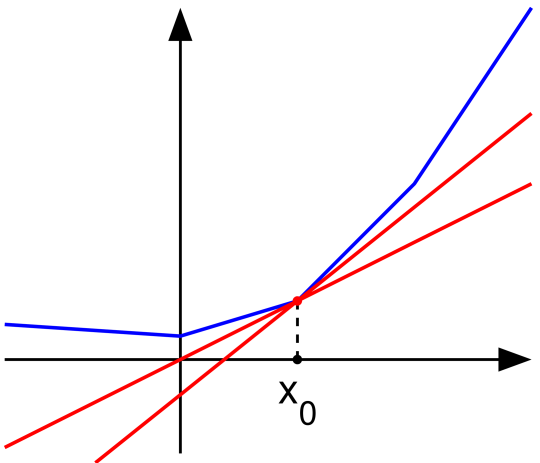
\includegraphics[scale=0.3]{img/Subderivative_illustration.png}
    \setlength{\abovecaptionskip}{0cm}
    \caption{An illustration of subgradient}
    \label{fig:subgradient}
\end{figure}

In the figure \ref{fig:subgradient}, the red lines give two feasible directions of the subgradient of the blue function at \(x_0\).

\begin{proposition}
    The subgradient of the nuclear norm at \(X_0\) is given by \cite{lewis2003mathematics},\cite{watson1992characterization}
    \[\partial \norm{X_0}_* = \left\{UV^T+W \mid W \textnormal{ and } X\textnormal{ have orthogonal row/column spaces and } \norm{W} \leqslant 1 \right\},\]
    where \(U\) and \(V\) are factors of SVD of \(X_0\), i.e. \(X_0=U\Sigma V^T.\)
\end{proposition}


\subsection{Projected subgradient methods}

Considering the affine equality constraint of low-rank optimization, the iteration method should satisfy
\[X_{k+1}= \Pi(X_k-s_k Y_k), \qquad Y_k \in \partial (\norm{X_k}_*),\]
where \(\Pi\) is the orthogonal projection onto the affine subspace defined by the linear constraints \(\mathcal{A}(X)=b\) and \(s_{k}>0\) is a stepsize parameter. Alternatively, since \(X_{k}\) is feasible, we can rewrite this as
\[
X_{k+1}=X_{k}-s_{k} \Pi_{\mathcal{A}} Y_{k},
\]
where \(\Pi_{\mathcal{A}}\) is the orthogonal projection onto \(\mathcal{N}(\mathcal{A})\).

To find a subgradient of \(X_k\) we may need to get the SVD of \(X_k\) by the above proposition, which is a quite hard task. However, we only need \(UV^T\) rather than the whole information of SVD. So we can use a iterative method to find \(UV^T\) as the "angular" factor of the polar decomposition.

\begin{proposition}
    Let the SVD of \(X\) is \(U\Sigma V^T\), then the polar decomposition of it can be written as \(X=\tilde{U} \tilde{P}\), where
    \[\tilde{U}=U V^T,\qquad \tilde{P}=V\Sigma V^T,\]
    satisfying that \(\tilde{U}\) is orthogonal and \(\tilde{P}\) is positive semidefinite.
\end{proposition}

This proposition shows that \(\tilde{U}\) is what we actually need.

We have some effective methods to get a numerical approximation of the polar decomposition, such as the \emph{Halley's method}\cite{nakatsukasa2010optimizing}
\[\tilde{U}_{n+1} = \tilde{U}_{n}\left(3 I+\tilde{U}_{n}^{T} \tilde{U}_{n}\right)\left(I+3 \tilde{U}_{n}^{T} \tilde{U}_{n}\right)^{-1}, \quad \tilde{U}_{0}=X_k.\] 
\subsection{Convergence analysis}
Regarding convergence, for most nonsmooth problems, subgradient methods do not guarantee that \(X_k\) can be arbitrarily close to the optimal point. There are several probabilities for choices of stepsize \(s_k\). The simplest choice that can guarantee convergence is to use a diminishing stepsize with an infinite travel condition, such as 
\[ \lim_{k\to \infty} s_k=0,\qquad \sum_{k>0}s_k\textnormal{ diverges}.\]

More recently, several nonlinear projected subgradient methods, under the rubric of \emph{mirror descent}, have been developed (e.g., by Nemirovski and Yudin \cite{blair1985problem}), followed by a subsequent rederivation and analysis by Beck and Teboulle \cite{beck2003mirror}. These algorithms, and their accompanying analysis, provide improved theoretical guarantees and practical performance over the standard Euclidean projected subgradient method described above. It would be of great interest to analyze to what extent these methods can be applied to the nuclear norm minimization problem.

In many scenarios, even the computation of an SVD or a Halley-like iteration can be too computationally expensive. Another method for  very large-scale problems is \emph{low-rank parametrization}, which  must give up guarantees of convergence for a high speed \cite{recht2010guaranteed}.

\section{Implementation}

\subsection{Code}

\subsection{Result}

\section{Conclusion}

\bibliographystyle{IEEEtran}

\bibliography{references.bib}

\end{document}